%\documentclass[10pt,a4paper]{article}
%\usepackage[utf8x]{inputenc}
%\usepackage[francais]{babel}
%\usepackage[T1]{fontenc}
%\usepackage{amsmath}
%\usepackage{verbatim}
%\usepackage{amsfonts}
%\usepackage{amssymb}
%\usepackage{graphicx}
%\usepackage{here}
%\usepackage{hyperref}
%\usepackage[left=2cm,right=2cm,top=2cm,bottom=2cm]{geometry}
%\newcommand{\HRule}{\rule{\linewidth}{0.5mm}}
%
%\usepackage{esvect} % Vecteurs
%\usepackage[amssymb]{SIunits}
%\usepackage{eurosym}
%\usepackage{mathrsfs}
%\usepackage{dcolumn}
%\usepackage{pifont}
%\usepackage{amsthm}
%
%
%%-------------------------------
%% TEST PACKAGES (GEO) POUR COMPILATION
%%-------------------------------
%\usepackage {lmodern}
%\usepackage{soul}
%\usepackage{fancyhdr} %un joli header
%\usepackage{enumerate}
%\usepackage{color}
%\usepackage{multicol}
%\usepackage{amsfonts}
%\usepackage{amsthm}
%\usepackage{mathrsfs}
%\usepackage{pifont}
%\usepackage{cancel}
%\usepackage{epstopdf}
%\usepackage{pifont}
%
%
%
%\title{CM7: LINMA 2471: Optimization methods and models: Lecture 7}
%\date{November, 4th 2015}
%\author{Ciamarra Geoffrey \and Losseau Bruno \and Lucas Joachim}
%
%\begin{document}
%\maketitle
%\selectlanguage{french}
%\theoremstyle{plain}
%\newtheorem{theorem}{Theorem}[section] % reset theorem numbering for each chapter
%\newtheorem{definition}{Definition}[section] % definition numbers are dependent on theorem numbers
%\newtheorem{example}{Example}[section] % same for example numbers
%
%\newtheorem{proposition}{Proposition}[section]
%\newtheorem{corollary}{Corollary}[section]
%\newtheorem{remark}{Remark}[section]

% Examples: \begin{example} .... \end{example}
% Definitions: \begin{definition} ... \end{definition}
% Theorems: \begin{theorem} ... \end{theorem}
% Propositions: \begin{proposition} ... \end{proposition}
% Remarks: \begin{remark} ... \end{remark}



\section{Conic optimization}
In order to introduce the conic optimization concept, let's begin with an linear example. 
\begin{example}[Linear optimisation problem]
\begin{leftbar}
\label{ex:C1}
\begin{align}
& & \nonumber \\ 
& \underset{y_i}{\max} \nonumber
& & 2y_1+3y_2+2y_3 \nonumber \\ 
& \text{subject to}
& & y_1 + y_2 \leq 1 \label{eq1} \\
& & & y_2 + y_3 \leq 2 \label{eq2} \\
& & & y_3 \leq 3 \label{eq3}
\end{align}

A feasible point is given by $(y_1,y_2,y_3)= (1,0,2)$ which provides a cost function value $6$. \\ \\ \textit{How to know whether $6$ is strictly lower than or strictly higher than or equal to the optimal objective value ?}  \\ \\ Since a feasible point gives $6$ as cost function value, the optimal objective value is not strictly lower than $6$. The value $6$ can be increased to $7$ by taking the feasible point $(y_1,y_2,y_3)= (2,-1,3)$. So the optimal objective value is not equal to $6$ but higher than $6$.\\ Concerning the value $7$, we could ask our question again,\textit{ how to prove that the optimal objective value is higher than or equal to $7$ ? } \\ \\ We need an upper bound on the value for the objective function. This can be achieved by taking a linear combination of the constraints. \\ \\ Indeed, 
\begin{align*}
2 \times \text{~constraint~} (\ref{eq1})+ 1 \times \text{~constraint~} (\ref{eq2})+ 1 \times \text{~constraint~}(\ref{eq3}) & = 2y_1+3y_2+2y_3 \\
& \leq 7
\end{align*}
$7$ is an upper bound for the objective value function. Since we have found a feasible point for which the objective value is equal to $7$, we can claim that the optimal objective value is equal to $7$. 
\end{leftbar}
\end{example}

It is possible to find a bound for the objective value for any linear problem. We want to extend the notion of linear problems while keeping their `nice' properties of linear problems (i.e. duality and efficient algorithms). In order to extend this notion, we will generalize the inequalities $\leq$ and $\geq$ in the linear problems. \\ \\
With $K \subseteq \mathbb{R}^n$, we define an generalized type of inequalities\[ a \succeq_K 0
 \Leftrightarrow a \in K \]
On the basis of this definition, we also have the following properties \begin{align*}
 a \succeq_K b \Leftrightarrow a-b \succeq_K 0
\Leftrightarrow a-b \in K \\ a \preceq_K b
\Leftrightarrow b \succeq_K a \Leftrightarrow b-a \succeq_K 0
\Leftrightarrow b-a \in K \end{align*}
Let us also impose two sensible properties for an order

\begin{property}
\label{Prop:C1}
$a \succeq_K 0 \Rightarrow \lambda a \succeq_K 0 \text{ for any } \lambda \ge 0$ 
\end{property}
\begin{property}
\label{Prop:C2}
$a \succeq_K 0 \text{ and } b \succeq_K 0 \Rightarrow a+b \succeq_K 0$
\end{property}
The Property \ref{Prop:C1} means that $K$ is a \emph{cone} and the Property \ref{Prop:C2} means that $K$ is \emph{closed under addition}.
The $K$ must be convex, $K$ is said to be a convex cone. In fact, for any cone $K$ (closed under non-negative scalar multiplication), we have the equivalence
\[ K \text{ is closed under addition } \Leftrightarrow K \text{ is convex} \]

\subsection{Generalization}
From the usual formulation of the problem, one can generalize: 
\begin{center}$\max b^Ty$ such that $A^Ty$ $\leqslant$ c \\
$\Downarrow$ \\
$\max b^Ty$ such that $A^Ty$ $\preceq_K$ c
\end{center}
This problem is convex.\\
Considering the standard linear case, $K = \mathbb{R}^n_+$.

\begin{example}
\begin{leftbar}
Going back to example \ref{ex:C1}, how would one define the set $K$?\\
As: 
\[A^T = \left( \begin{array}{ccc}
1 & 1 & 0 \\
0 & 1 & 1 \\
0 & 0 & 1 \end{array} \right), \hspace{1cm}
C = \left( \begin{array}{c}
1 \\
2 \\
3 \end{array} \right) \]
Defining $K = \mathbb{R}^3_+$ implies: 
\[C-A^Ty = 
\left( \begin{array}{c}
1 \\
2 \\
3 \end{array} \right)-
\left( \begin{array}{ccc}
1 & 1 & 0 \\
0 & 1 & 1 \\
0 & 0 & 1 
\end{array} \right) y
\subset K = \mathbb{R}^3_+ 
\]

\[\left( \begin{array}{c}
1 - y_1 - y_2 \\
2 - y_2 - y_3\\
3 - y_3 \end{array} \right) 
\subset K = \mathbb{R}^3_+ 
\]
\end{leftbar}
\end{example}

\subsection{Solving a problem on different cones}
As one consider polyhedron cones, the boundary is linear. Also, applying a linear operation to a linear problem keeps the problem linear. 
As a result, applying a rotation or a scaling operation to a cone and solving the problem on the newly obtained cone is equivalent to solving it on the first cone. \label{solving_diff_cones}
\begin{center}
\begin{figure}[h]
\centering
  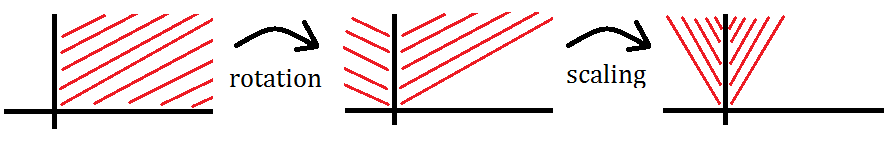
\includegraphics[scale=0.6]{images/Course7_equivalenceCones.png}\\
   \label{bruno}
  \caption{Solving a problem on one cone is equivalent to solve it on a newly obtained cone via rotation and scaling.}
\end{figure}
\end{center}

The conic optimization is useful since it is more general than linear optimization. The sets considered are not polyhedrons anymore but rather curved sets. Thus, it can cover more problems.

\subsection{Lorentz cone}
A common example of a cone is the Lorentz cone or ice cream cone. It is defined such as: 
\[
\mathbb{L}^n = \{(x_0,\dots, x_n) \in \mathbb{R}^{n+1} \mid \sqrt{x_1^2+...+x_n^2} \le x_0 \}
\]

One can verify it is indeed a cone by checking that when multiplying a value in the cone by a scalar it stays in the cone; and that addition is preserved (intuition: rule of parallelogram). Also, checking if the hull is a cone is the same as checking whether it is convex or not.

\begin{example}
\begin{leftbar}
Let the problem:
\begin{center}
$\max (y_1+y_2)$ \\
$y_1^2+y_2^2 \leq 7$
\end{center}

One notes that the constraint is quadratic and semi-definite positive. One would like to formulate the problem as linear, except for the cone. All that is non-linear shall be put in the cone, hence: 

\begin{align*}
y_1^2+y_2^2 \leq 7 \, 
\Leftrightarrow \, 
\sqrt{y_1^2+y_2^2} \leq \sqrt{7} \\ \vspace{0.5cm}
\Updownarrow \\ \vspace{0.5cm}
\left( \begin{array}{c}
\sqrt7 \\
y1\\
y2 \end{array} \right) 
\in \mathbb{L}^2 \
\Leftrightarrow \, 
\
\left( \begin{array}{c}
\sqrt7 \\
y1\\
y2 \end{array} \right) 
\succeq_{ \mathbb{L}^2}
\left( \begin{array}{c}
0\\
0\\
0\\\end{array} \right) \\ \vspace{0.5cm}
\Updownarrow \\ \vspace{0.5cm}
\left( \begin{array}{c}
\sqrt7 \\
0\\
0 \end{array} \right) 
\succeq_{ \mathbb{L}^2}
\left( \begin{array}{c}
0 \\
-y_1\\
-y_2 \end{array} \right) 
\end{align*} 

Finally:

\begin{center}
\[
C =\sqrt7, 
\hspace{1cm}
A = \left( \begin{array}{cc}
-1 & 0 \\
0 & -1 \end{array} \right), 
\hspace{1cm}
y = \left( \begin{array}{c}
y_1 \\
y_2 \end{array} \right)
\]
\end{center}
And the problem can be written as: 
\begin{center}
$\max (y_1+y_2)$ \\
$-y_1-y_2 \preceq_{\mathbb{L}^2} \sqrt7$
\end{center}
\end{leftbar}
\end{example}

\subsection{Requirements for $K$} 
\begin{enumerate}
\item $x \succeq 0$ and $x \preceq 0 \Rightarrow x = 0$

which means $K \cap (-K) = \{ 0 \}$ (the cone is \emph{pointed})

\item We define the strict inequality by $a \succ 0
\Leftrightarrow a \in int ~K$ (and $a \succ b$ iff $a-b \in int~
K$)

Hence we require $int~ K \neq \emptyset$ (the cone is
\emph{solid})

\item Finally, we would like to be able to take limits:
\[ \text{If } \{ x_i \}_{i \to \infty} \text{ with } x_i \succeq_K
0 \ \forall i,\ \text{then} \lim_{i \to \infty} x_i = \bar{x}
\Rightarrow \bar{x} \succeq_K 0 \] which is equivalent to saying
that $K$ is \emph{closed}. \end{enumerate} 


A convex cone $K$ that is solid, pointed and closed will be called a \emph{proper cone}.\\

As seen in section \ref{solving_diff_cones}, in the conic optimization theory, all the cones can always be merged as an only one according to the following definition.\\

\begin{definition} 
Considering several conic constraints \[ A_1^T y \preceq_{K_1} c_1
\text{ and } A_2^T y \preceq_{K_2} c_2 \] which are equivalent to
\[ c_1 - A_1^T y \in K_1 \text{ and } c_2 - A_2^T y \in K_2 \] one
introduces the product cone $K = K_1 \times K_2$ to write
\[ (c_1 - A_1^T y, c_2 - A_2^T y) \in K_1 \times K_2
\] \[ \Leftrightarrow \begin{pmatrix} c_1 \\ c_2
\end{pmatrix} -
\begin{pmatrix} A_1^T \\ A_2^T \end{pmatrix} \in K_1 \times K_2
\Leftrightarrow
 \begin{pmatrix} c_1 \\ c_2 \end{pmatrix} -
\begin{pmatrix} A_1^T \\ A_2^T \end{pmatrix} \succeq_{K_1 \times K_2} 0 \]
If $K_1$ and $K_2$ are proper, $K_1 \times K_2$ is also proper.
\end{definition}

However, in this course, and for the exercises, we will not merge the cones.

\subsection{Equivalence with convex optimization} 
Since a cone is convex, conic optimization can be related to convex optimization: conic optimization is clearly a special case of convex optimization. What about the reverse statement ?

\[ \min_{x \in \mathbb{R}^n} f(x) \text{ such that } x \in X \subseteq
\mathbb{R}^n \]

\begin{itemize}
\item The objective of a convex problem can be assumed
\emph{w.l.o.g.}\footnote{without loss of generality} to be \emph{linear}: $f(x) = c^T x$

\item The feasible region of a convex problem can be assumed
\emph{w.l.o.g.} to be in the \emph{conic} standard format: \[ X
= \{ x \in K \text{ and } A x = b \} \]
\end{itemize}

$\Rightarrow$ conic optimization \emph{equivalent} to convex
optimization. \\

One can prove that everything in the use of conic optimization, must be convex. Considering the conic constraint: 
\begin{equation}
c-A^Ty \in K \nonumber 
\end{equation}
choosing $K$ to be convex is a good way to ensure the constraint to be convex too since linear transformations preserve convexity. \\

\section{Duality}
What about the conic dual problems ? Since we generalized
\[ \max b^T y \text{ s.t. } A^T y \leq c \] to
\[ \max b^T y \text{ s.t. } A^T y \preceq_K c \] it could be tempting to generalize
\[ \min c^T x \text{ s.t. } Ax = b \text{ and } x \geq 0 \]
to
\[ \min c^T x \text{ s.t. } Ax = b \text{ and } x \succeq_K 0 .\]
However, this is not the right primal-dual pair ! Actually, we must also dualize the cone; and the corresponding correct primal-dual pair is given by 
\vspace{0.3cm} \[ \max b^T y \text{ such that } A^T y \preceq_K c \]
\[ \min c^T x \text{ such that } Ax = b \text{ and } x \succeq_{K^*} 0 \]

\vspace{0.3cm}
where we introduce the dual cone $K^*$ defined as 
\[ K^* = \{ z \in \mathbb{R}^n \text{ such that }
x^T z \geq 0 \ \forall x \in K \} \]

\begin{itemize}
\item $K^*$ is a convex cone, called the \emph{dual} cone of $K$;
\item $K^*$ is always \emph{closed}, and if $K$ is closed, $(K^*)^* = K$; \item $K$ is \emph{pointed} (resp. 
   solid) $\Rightarrow K^*$ is \emph{solid} (resp. pointed) \item Cartesian products: $(K_1 \times K_2)^*
   = K_1^* \times K_2^*$;
\item $(\mathbb{R}^n+)^* = \mathbb{R}^n+, (\mathbb{L}^n)^* = \mathbb{L}^n, (\mathbb{S}_+^n)^* = \mathbb{S}_+^n$: these cones are self-dual, but there are (many) cones which are not.
\end{itemize}


% \end{document}
